\documentclass[table]{beamer}

% Use metropolis theme
\usepackage[progressbar=foot]{theme/beamerthememetropolis}
\usepackage{amsmath}
\usepackage{marvosym}
\usepackage{xcolor}
\usepackage{minted}

\title{Using Neural Networks for Time-Series Prediction}

\date{\today}
\author{Joe Jevnik}
\institute{PyData NYC 2017}

\begin{document}
\maketitle

\begin{frame}{Outline}
  \begin{enumerate}
  \item Introduce problem
  \item Phrase problem as an ML problem
  \item Collect and apply data
  \item Select features
  \item Train the model
  \item Improve the model
  \item Tips
  \end{enumerate}
\end{frame}

\begin{frame}{Who am I?}
  \begin{columns}
    \column{0.35\textwidth}
    \begin{center}
      
\includegraphics[width=0.90\textwidth]{images/quantopian.png}
    \end{center}

    \column{0.6\textwidth}
    \begin{itemize}
    \item Works with storage and manipulation of time series data
    \item Integrates third-party data sets
    \end{itemize}
  \end{columns}
\end{frame}

\section{The Problem}

\begin{frame}{Osu!}
  \begin{center}
    
\includegraphics[width=0.60\textwidth]{images/osu-logo.png}
  \end{center}
\end{frame}

\begin{frame}[fragile]{Elements}
  \begin{columns}[c]
    \column{0.33\textwidth}
    \only<1->{
      \begin{figure}
        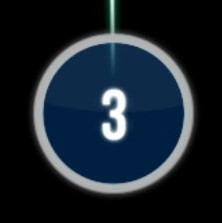
\includegraphics[width=0.8\textwidth]{images/circle.jpg}
        \caption{A hit circle}
      \end{figure}
    }
    
    \column{0.33\textwidth}
      \only<2->{
        \begin{figure}
          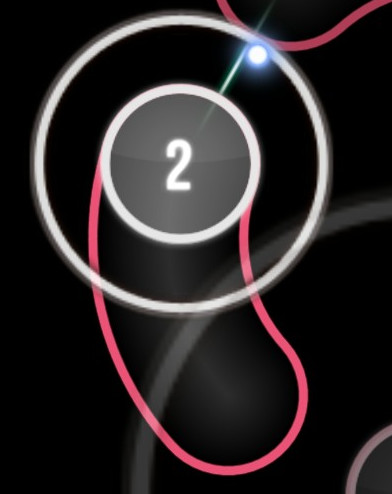
\includegraphics[width=0.8\textwidth]{images/slider.jpg}
          \caption{A slider}
        \end{figure}
      }

    \column{0.33\textwidth}
    \only<3->{
      \begin{figure}
        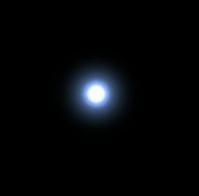
\includegraphics[width=0.8\textwidth]{images/cursor.jpg}
        \caption{Mouse cursor}
      \end{figure}
    }
  \end{columns}
\end{frame}

\begin{frame}{Osu! (cont.)}
  \begin{block}{Scoring}
    \begin{itemize}
    \item[]<1-> 300 points if on the beat
    \item[]<2-> 100 points if slightly off the beat
    \item[]<3-> 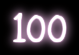
\includegraphics[width=0.12\textwidth]{images/hit100.png}
    \item[]<4-> 50 points if really off the beat
    \item[]<5-> 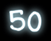
\includegraphics[width=0.12\textwidth]{images/hit50.png}
    \item[]<6-> 0 points for missing entirely
    \item[]<7-> 
\includegraphics[width=0.12\textwidth]{images/hit0.png}
    \end{itemize}
  \end{block}
\end{frame}

\begin{frame}{Osu! (cont.)}
  \begin{block}{Sample}
    \texttt{\$ mpv videos/osu-example.avi}
  \end{block}
\end{frame}

\begin{frame}{Problem}
  \begin{itemize}
  \item[]<1-> Improve my rank quickly
  \item[]<2-> Many new songs a week
  \item[]<3-> Particular playstyle
  \item[]<4-> Arbitrage opportunity?
  \end{itemize}
\end{frame}

\section{Phrasing the Problem}

\begin{frame}{Problem}
  \begin{block}{Predict my score on a beatmap}
    \begin{itemize}
    \item[]<2-> Need to compute accuracy \%
    \item[]<3-> Temporal Accuracy
    \item[]<4-> Aim Accuracy
    \end{itemize}
  \end{block}
\end{frame}

\begin{frame}{Machine Learning Models}
  \only<1>{
    \begin{block}{Classifiers}
      Label a sample as a member of one of a finite set of classes.
    \end{block}
  }
  \only<2>{
    \begin{block}{Regressors}
      Approximate a numerical function.
    \end{block}
  }
\end{frame}

\begin{frame}{LSTM Models}
  \begin{itemize}
  \item[]<1-> Order dependent data
  \item[]<2-> Sequence of observations
  \item[]<3-> Uses windows of time-sorted observations
  \end{itemize}
\end{frame}

\begin{frame}{Our Problem}
  For each hit-object, predict..

  \vspace{\fill}

  \begin{columns}[T]
    \column{0.35\textwidth}
    \only<2->{
      \begin{block}{Classifier}
        A label.

        \begin{itemize}
        \item 300
        \item 100
        \item 50
        \item 0 (miss)
        \end{itemize}
      \end{block}
    }

    \column{0.55\textwidth}
    \only<3>{
      \begin{block}{Regressor}
        A numeric error metric.

        \begin{enumerate}
        \item Aim Error ((x, y) error)
        \item Accuracy Error (punctuality)
        \end{enumerate}
      \end{block}
    }
  \end{columns}
\end{frame}

\section{Data Collection}

\begin{frame}{Beatmaps}
  \begin{itemize}
  \item[]<1-> Hit objects in (x, y, time) space.
  \item[]<2-> Circle Size (CS)
  \item[]<3-> Approach Rate (AR)
  \item[]<4-> Overall Difficulty (OD) (score thresholds)
  \end{itemize}
\end{frame}

\begin{frame}[fragile, label=raw-data]{Raw Data}
  \begin{block}{Beatmap}
    \begin{verbatim}
[HitObjects]
103,272,52926,6,0,L|111:176,1,67.5000025749208
93,95,53279,1,2,0:3:0:0:
194,131,53455,2,0,B|263:160|264:100|337:135,1,135.000005149842,0|2,0:0|0:3,0:0:0:0:
437,204,53985,2,0,L|432:286,1,67.5000025749208
394,105,54338,6,0,L|399:17,1,67.5000025749208
286,62,54690,1,2,0:3:0:0:
177,54,54867,2,0,B|110:74|110:30|41:53,1,135.000005149842,0|2,0:0|0:3,0:0:0:0:
70,213,55396,2,0,L|77:132,1,67.5000025749208
161,215,55749,6,0,P|175:273|247:314,1,135.000005149842,0|2,0:0|0:3,0:0:0:0:
341,286,56279,1,0,0:0:0:0:
308,183,56455,2,0,P|268:201|245:238,1,67.5000025749208,0|2,0:0|0:3,0:0:0:0:
    \end{verbatim}
  \end{block}
\end{frame}

\begin{frame}{Mods}
  \begin{itemize}
  \item<1-> Hard Rock (HR)
  \item<2-> Double Time (DT)
  \item<3-> Hidden (HD)
  \item<4-> etc...
  \end{itemize}
\end{frame}

\begin{frame}{Replays}
  \only<1-3>{
    \begin{block}{Time series of...}
      \begin{itemize}
      \item[]<2-> Cursor location
      \item[]<3-> Keyboard state
      \end{itemize}
    \end{block}
  }

  \only<4>{
    I had about seven years of replays laying around!
  }
\end{frame}

\begin{frame}[label=od-table]{Understanding our data}
  \begin{block}{Accuracy thresholds (milliseconds)}
    \begin{center}
      \begin{tabular}{r | r r r}
        OD & 300 & 100 & 50 \\
        \hline
        1 & 73.5 & 131.5 & 189.5 \\
        2 & 67.5 & 123.5 & 179.5 \\
        3 & 61.5 & 115.5 & 169.5 \\
        4 & 55.5 & 107.5 & 159.5 \\
        5 & 49.5 & 99.5 & 149.5 \\
        6 & 43.5 & 91.5 & 139.5 \\
        7 & 37.5 & 83.5 & 129.5 \\
        8 & 31.5 & 75.5 & 119.5 \\
        9 & 25.5 & 67.5 & 109.5 \\
        10 & 19.5 & 59.5 & 99.5
      \end{tabular}
    \end{center}
  \end{block}
\end{frame}

\begin{frame}{Understanding our data (cont.)}
  \begin{center}
    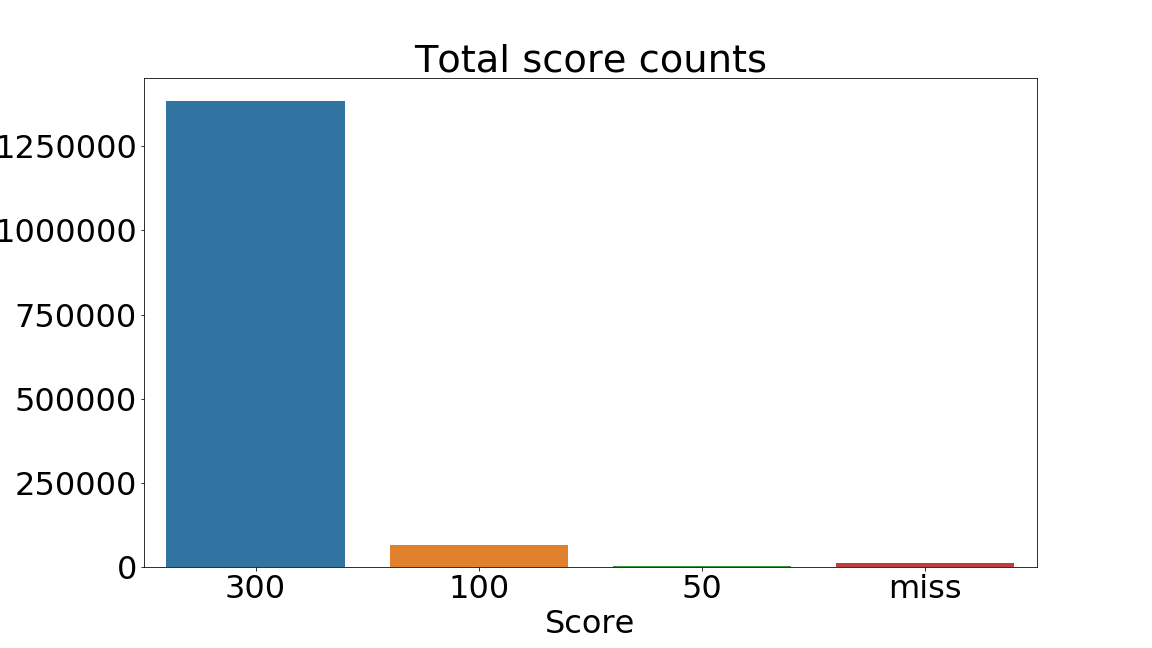
\includegraphics[width=1.00\textwidth]{images/hit-counts.png}
  \end{center}
\end{frame}

\begin{frame}{Prediction Targets}
  \only<1-3>{
    \begin{block}{Joining Data}
      \begin{itemize}
      \item[]<2-> Find all clicks by taking times where key state changes
      \item[]<3-> Match click with the nearest hit object (ignores hit locking!)
      \end{itemize}
    \end{block}
  }

  \only<4-5>{
    \begin{block}{Accuracy Error}
      \begin{itemize}
      \item[]<4-> Absolute difference in time.
      \item[]<5-> Comparable across different OD
      \end{itemize}
    \end{block}
  }

  \only<6-7>{
    \begin{block}{Aim Error}
      \begin{itemize}
      \item[]<6-> Euclidean distance between click and center of circle.
      \item[]<7-> Comparable across different CS
      \end{itemize}
    \end{block}
  }
\end{frame}

\section{Feature Selection}

\begin{frame}{What is a feature?}
  Numeric inputs to the ML model

  \begin{enumerate}
  \item[]<2-> What are we observing
  \item[]<3-> Focus the model on aspects of the data
  \item[]<4-> Chance to use domain knowledge
  \end{enumerate}
\end{frame}

\againframe{raw-data}

\begin{frame}{Simple Features}
  \begin{enumerate}
  \item[] \texttt{absolute\_x}
  \item[] \texttt{absolute\_y}
  \item[] \texttt{absolute\_time}
  \end{enumerate}
\end{frame}

\begin{frame}{Domain Specific Features}
  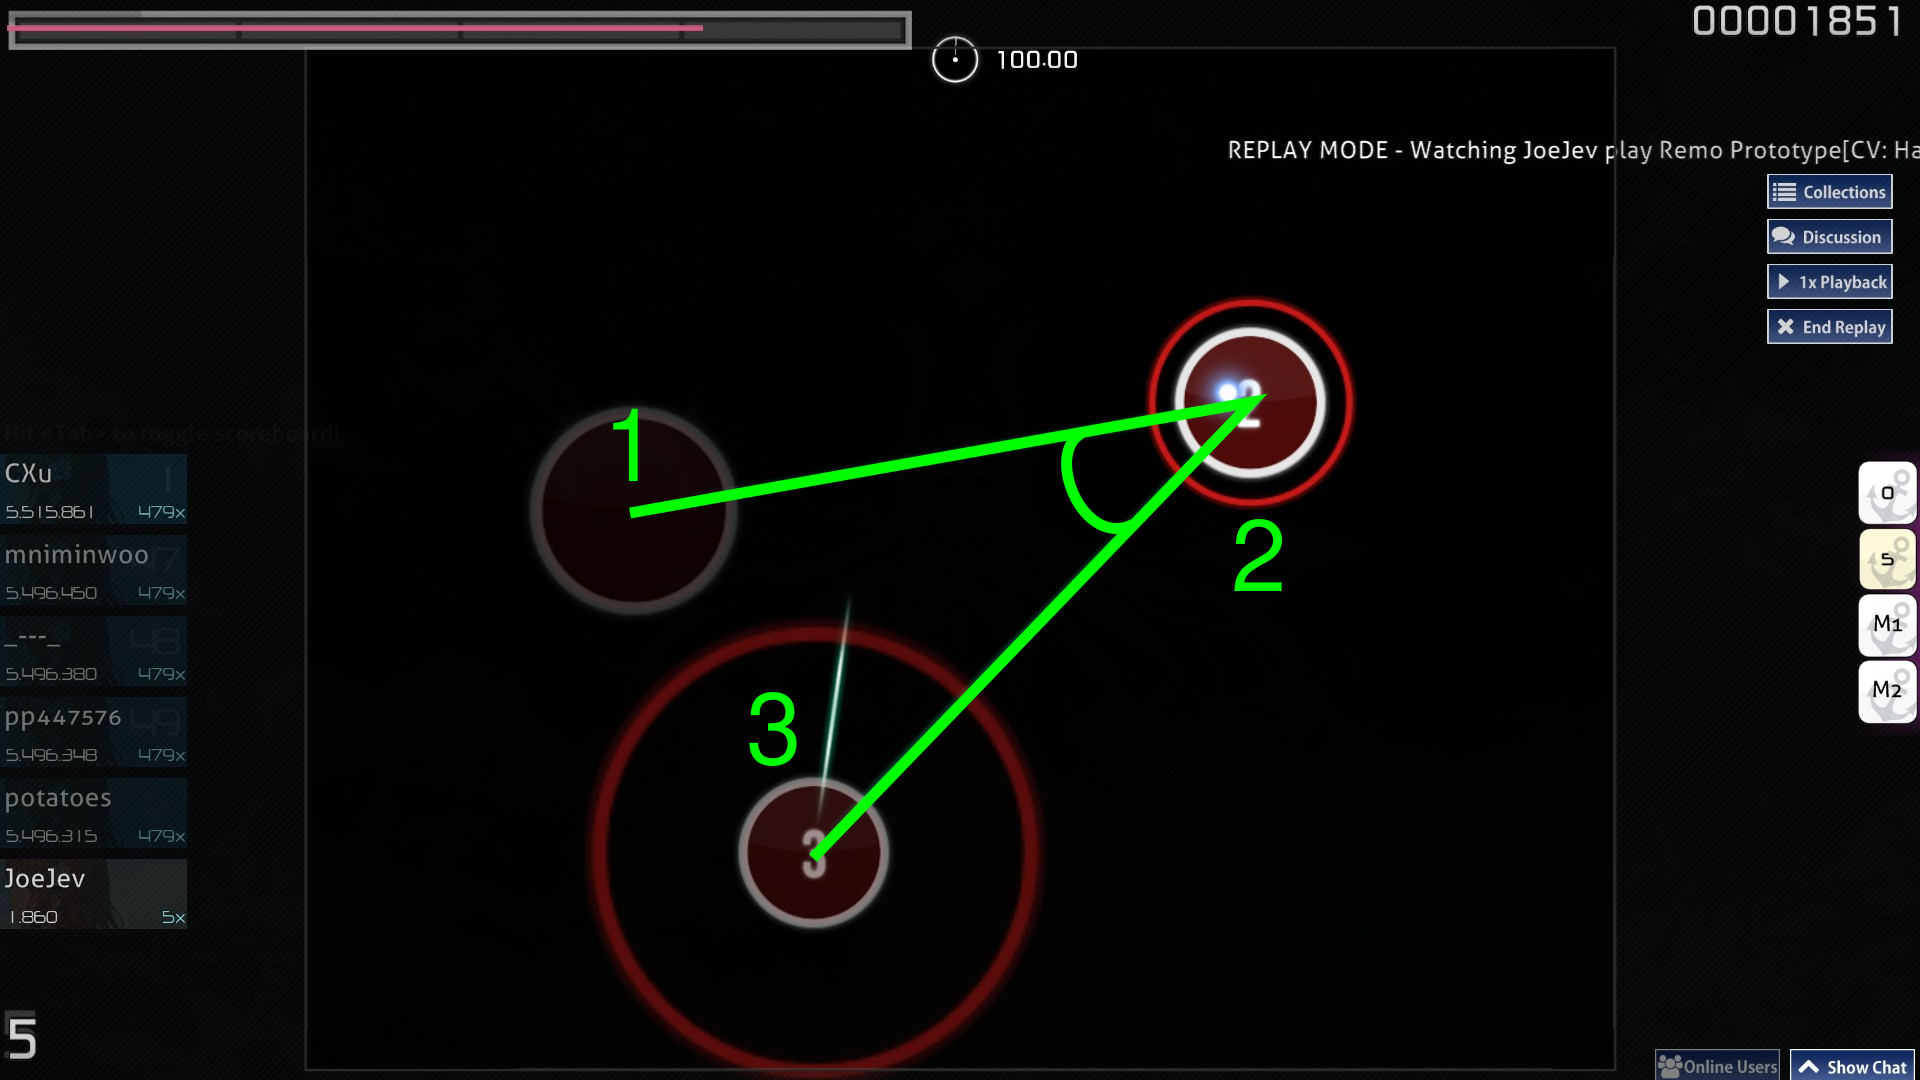
\includegraphics[width=1.00\textwidth]{images/angle.png}
\end{frame}

\begin{frame}{Windows}
  \only<1>{
    \begin{center}
      \begin{tabular}{r r r}
        time & x & y \\
        \hline
        00:37.366 & 372 & 94 \\
        00:37.763 & 447 & 205 \\
        00:38.027 & 217 & 299 \\
        00:38.291 & 229 & 171 \\
        00:38.424 & 274 & 358 \\
        00:38.688 & 149 & 221 \\
        00:38.952 & 330 & 186 \\
        00:39.217 & 233 & 127 \\
        00:39.481 & 233 & 127 \\
        00:39.613 & 198 & 303
      \end{tabular}
    \end{center}
  }
  
  \only<2>{
    \begin{center}
      \begin{tabular}{r r r}
        time & x & y \\
        \hline
        00:37.366 & 372 & 94 \\
        00:37.763 & 447 & 205 \\
        00:38.027 & 217 & 299 \\
        00:38.291 & 229 & 171 \\
        00:38.424 & 274 & 358 \\
        \rowcolor{blue!25} 00:38.688 & 149 & 221 \\
        00:38.952 & 330 & 186 \\
        00:39.217 & 233 & 127 \\
        00:39.481 & 233 & 127 \\
        00:39.613 & 198 & 303
      \end{tabular}
    \end{center}
  }

  \only<3>{
    \begin{center}
      \begin{tabular}{r r r}
        time & x & y \\
        \hline
        00:37.366 & 372 & 94 \\
        \rowcolor{cyan!25} 00:37.763 & 447 & 205 \\
        \rowcolor{cyan!25} 00:38.027 & 217 & 299 \\
        \rowcolor{cyan!25} 00:38.291 & 229 & 171 \\
        \rowcolor{cyan!25} 00:38.424 & 274 & 358 \\
        \rowcolor{blue!25} 00:38.688 & 149 & 221 \\
        \rowcolor{cyan!25} 00:38.952 & 330 & 186 \\
        \rowcolor{cyan!25} 00:39.217 & 233 & 127 \\
        00:39.481 & 233 & 127 \\
        00:39.613 & 198 & 303
      \end{tabular}
    \end{center}
  }

  \only<4>{
    \begin{center}
      \begin{tabular}{r r r | r r}
        time & x & y & relative x & relative y\\
        \hline
        00:37.366 & 372 & 94 & - & - \\
        \rowcolor{cyan!25} 00:37.763 & 447 & 205 & 298 & -16 \\
        \rowcolor{cyan!25} 00:38.027 & 217 & 299 & 68 & 78 \\
        \rowcolor{cyan!25} 00:38.291 & 229 & 171 & 80 & -50 \\
        \rowcolor{cyan!25} 00:38.424 & 274 & 358 & 125 & 137 \\
        \rowcolor{blue!25} 00:38.688 & 149 & 221 & 0 & 0 \\
        \rowcolor{cyan!25} 00:38.952 & 330 & 186 & 181 & -35 \\
        \rowcolor{cyan!25} 00:39.217 & 233 & 127 & 84 & -94 \\
        00:39.481 & 233 & 127 & - & - \\
        00:39.613 & 198 & 303 & - & -
      \end{tabular}
    \end{center}
  }

  \only<5>{
    \begin{center}
      \begin{tabular}{r r r | r r}
        time & x & y & relative x & relative y\\
        \hline
        00:37.366 & 372 & 94 & - & - \\
        00:37.763 & 447 & 205 & - & - \\
        \rowcolor{cyan!25} 00:38.027 & 217 & 299 & -113 & 113 \\
        \rowcolor{cyan!25} 00:38.291 & 229 & 171 & -101 & -15 \\
        \rowcolor{cyan!25} 00:38.424 & 274 & 358 & -56 & 172 \\
        \rowcolor{cyan!25} 00:38.688 & 149 & 221 & -181 & 35 \\
        \rowcolor{blue!25} 00:38.952 & 330 & 186 & 0 & 0 \\
        \rowcolor{cyan!25} 00:39.217 & 233 & 127 & -97 & -59 \\
        \rowcolor{cyan!25} 00:39.481 & 233 & 127 & -97 & -59 \\
        00:39.613 & 198 & 303 & - & -
      \end{tabular}
    \end{center}
  }

  \only<6>{
    \begin{center}
      \begin{tabular}{r r r | r r}
        time & x & y & relative x & relative y\\
        \hline
        00:37.366 & 372 & 94 & - & - \\
        00:37.763 & 447 & 205 & - & - \\
        00:38.027 & 217 & 299 & - & - \\
        \rowcolor{cyan!25} 00:38.291 & 229 & 171 & -4 & 44 \\
        \rowcolor{cyan!25} 00:38.424 & 274 & 358 & 41 & 231 \\
        \rowcolor{cyan!25} 00:38.688 & 149 & 221 & -84 & 94 \\
        \rowcolor{cyan!25} 00:38.952 & 330 & 186 & 97 & 59 \\
        \rowcolor{blue!25} 00:39.217 & 233 & 127 & 0 & 0 \\
        \rowcolor{cyan!25} 00:39.481 & 233 & 127 & 0 & 0 \\
        \rowcolor{cyan!25} 00:39.613 & 198 & 303 & -35 & 176
      \end{tabular}
    \end{center}
  }
\end{frame}

\begin{frame}{Osu! Features}
  \begin{columns}[T]
    \column{0.35\textwidth}
    \begin{itemize}
    \item \texttt{absolute\_x}
    \item \texttt{absolute\_y}
    \item \texttt{absolute\_time}
    \item \texttt{relative\_x}
    \item \texttt{relative\_y}
    \item \texttt{relative\_time}
    \end{itemize}

    \column{0.5\textwidth}

    \begin{itemize}
    \item \texttt{is\_slider\_tick}
    \item \texttt{approach\_rate}
    \item \texttt{distance\_from\_previous}
    \item \texttt{distance\_to\_next}
    \item \texttt{pitch}
    \item \texttt{roll}
    \item \texttt{yaw}
    \end{itemize}
  \end{columns}
\end{frame}

\section{Training}

\begin{frame}{Input Shapes}
  \begin{block}{Feature array shape}
    \vspace{\fill}
    \begin{tabular}{r r r r r}
      $$($$ &
        \onslide<4->{number of windows}, &
        \onslide<3->{window length}, &
        \onslide<2->{number of features}, &
        $$)$$ \\
    \end{tabular}
  \end{block}

  \onslide<5->{
    \begin{block}{Label array shape}
      \vspace{\fill}
      \begin{tabular}{r r r}
        $$($$ & number of windows, & $$)$$ \\
        $$($$ & number of windows, & $$)$$ \\
      \end{tabular}
    \end{block}
  }
\end{frame}

\begin{frame}[fragile]{Keras}
  \begin{itemize}
  \item[]<1-> \begin{minted}{python}
input_ = keras.layers.Input(
    shape=(window_length, len(features))
)
    \end{minted}
  \item[]<2-> \begin{minted}{python}
lstm = keras.layers.LSTM(lstm_layer_size)(input_)
    \end{minted}
  \item[]<3-> \begin{minted}{python}
aim_error = keras.layers.Dense(
    1,
    activation='linear',
    name='aim_error',
)(lstm)
    \end{minted}
  \item[]<4-> \begin{minted}{python}
accuracy_error = keras.layers.Dense(
    1,
    activation='linear',
    name='accuracy_error',
)(lstm)
    \end{minted}
  \end{itemize}
\end{frame}

\begin{frame}[fragile]{Keras (cont.)}
  \begin{itemize}
  \item[]<1-> \begin{minted}{python}
model = keras.models.Model(
    inputs=input_,
    outputs=[aim_error, accuracy_error],
)
    \end{minted}
  \item[]<2-> \begin{minted}{python}
model.compile(
    loss='mse',
    optimizer='rmsprop',
)
    \end{minted}
  \end{itemize}
\end{frame}

\begin{frame}[fragile]{Keras (cont.)}
  \begin{itemize}
  \item[]<1-> \begin{minted}{python}
# compute features, aim_error, accuracy_error
model.fit(
    features,
    {
        'aim_error': aim_error,
        'accuracy_error': accuracy_error,
    },
)
    \end{minted}
  \item[]<2-> \begin{minted}{python}
model.predict(features)
    \end{minted}
  \end{itemize}
\end{frame}

\begin{frame}{How does it look?}
  \only<2>{
    bad
  }
\end{frame}

\begin{frame}{Feature Scaling}
  \begin{itemize}
  \item[]<1-> Sensitive to input ranges
  \item[]<2-> \texttt{(data - data.mean()) / data.std()}
  \item[]<3-> Save the mean and std of the training data!
  \end{itemize}
\end{frame}

\begin{frame}[fragile]{Data (again)}
  \begin{columns}[T]
    \column{0.65\textwidth}
    \begin{verbatim}
features:
    absolute_x:
      mean: 256.93
      std:  581144.54
      min:  -26.25
      max:  42978020236964152.0
    absolute_y:
      mean: 188.67
      std:  96280.10
      min:  -12.20
      max:  10754663190171874.0
    \end{verbatim}

    \column{0.35\textwidth}
    \only<2>{
      osu! playfield: \\ (512, 384)
    }
  \end{columns}
\end{frame}

\begin{frame}{Slider Curves}
  \only<1>{
    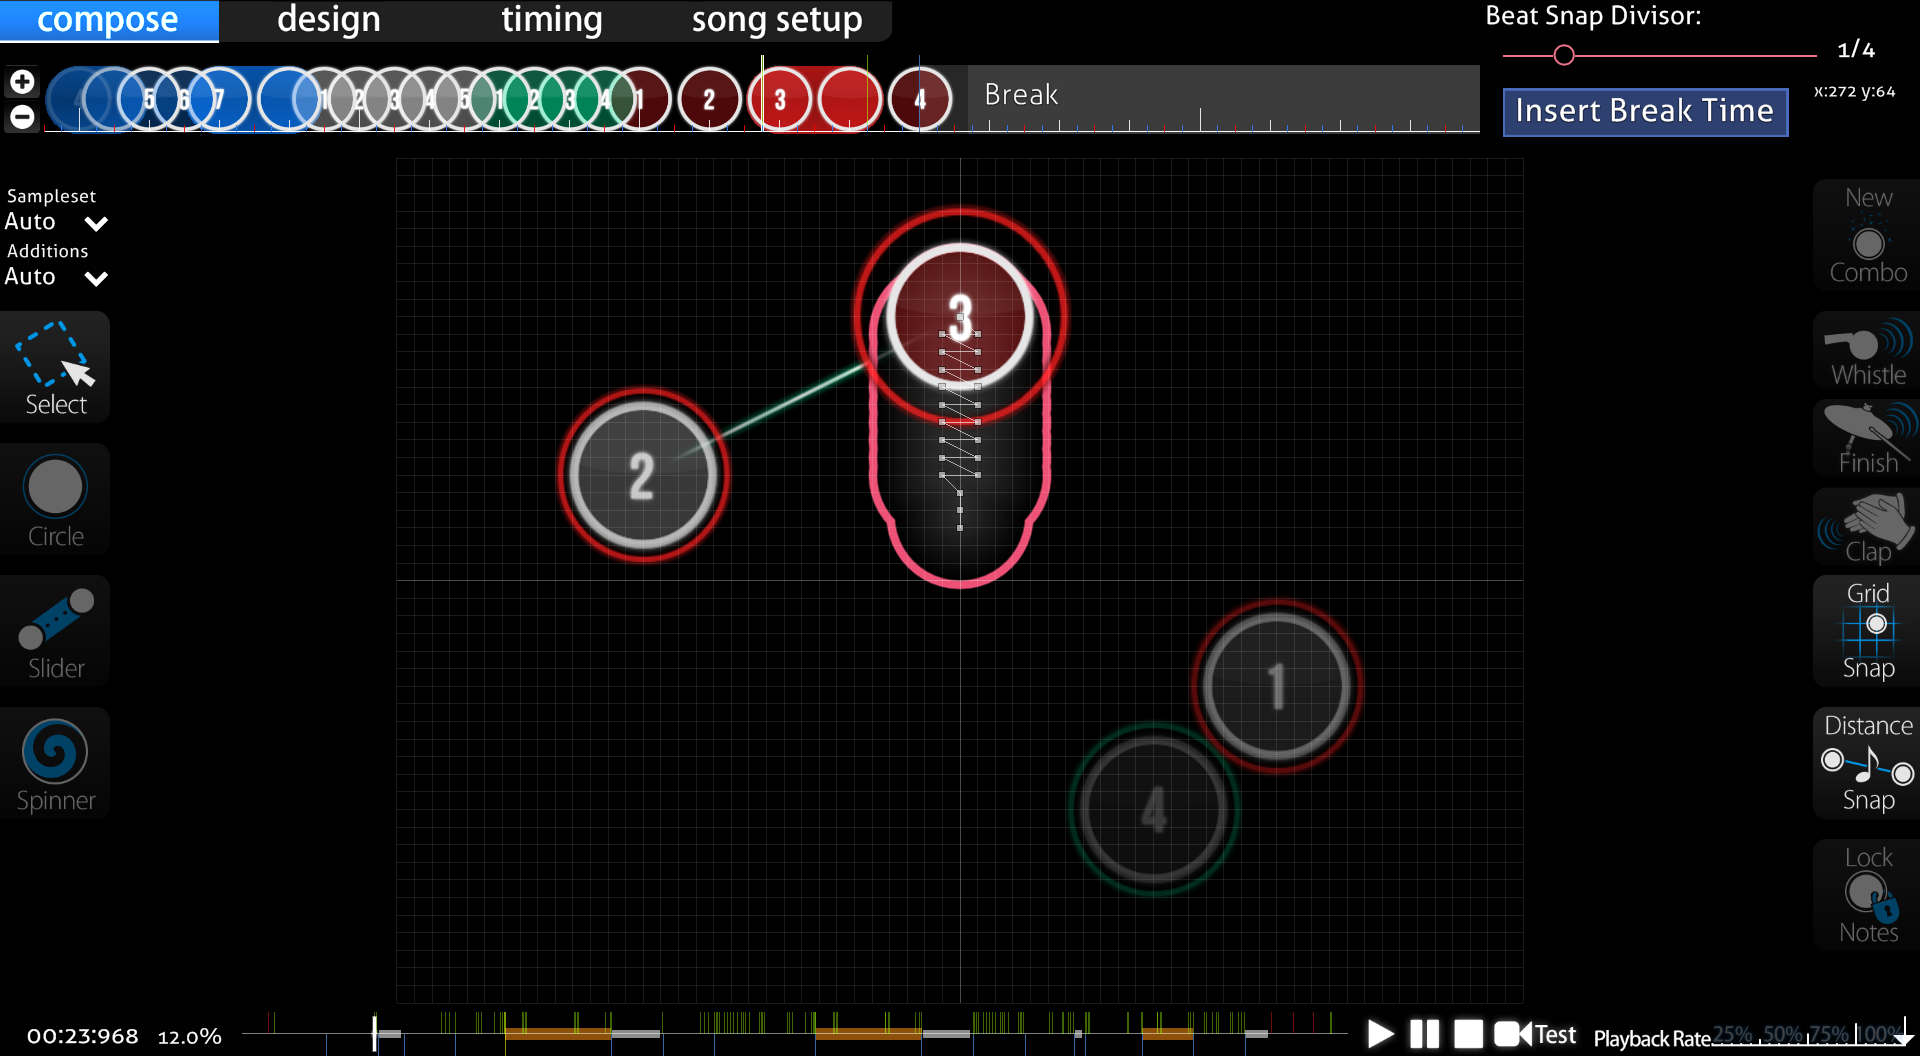
\includegraphics[width=1.00\textwidth]{images/slider-editor.png}
  }

  \only<2>{
    \begin{center}
      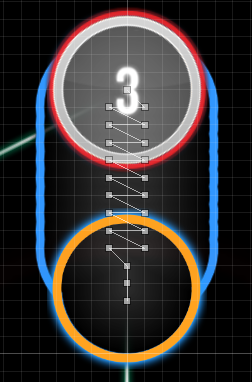
\includegraphics[height=0.8\textheight]{images/slider-close-up.png}
    \end{center}
  }

  \only<3>{
    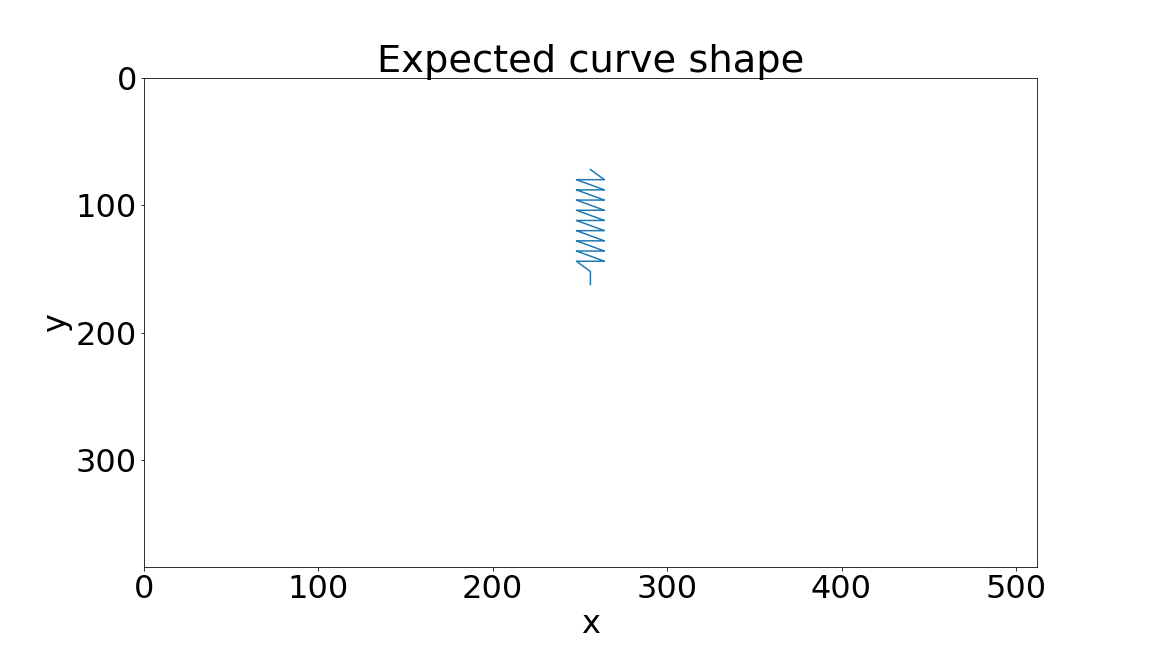
\includegraphics[width=1.00\textwidth]{images/expected-curve.png}
  }
  
  \only<4>{
    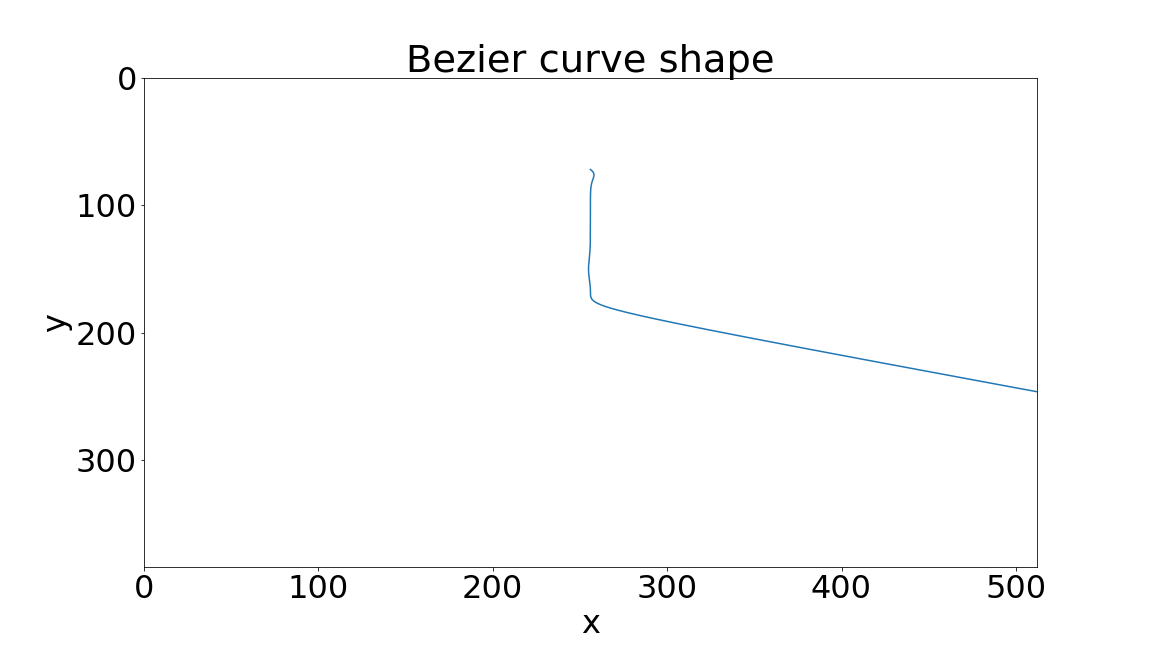
\includegraphics[width=1.00\textwidth]{images/bezier-curve-1.png}
  }

  \only<5>{
    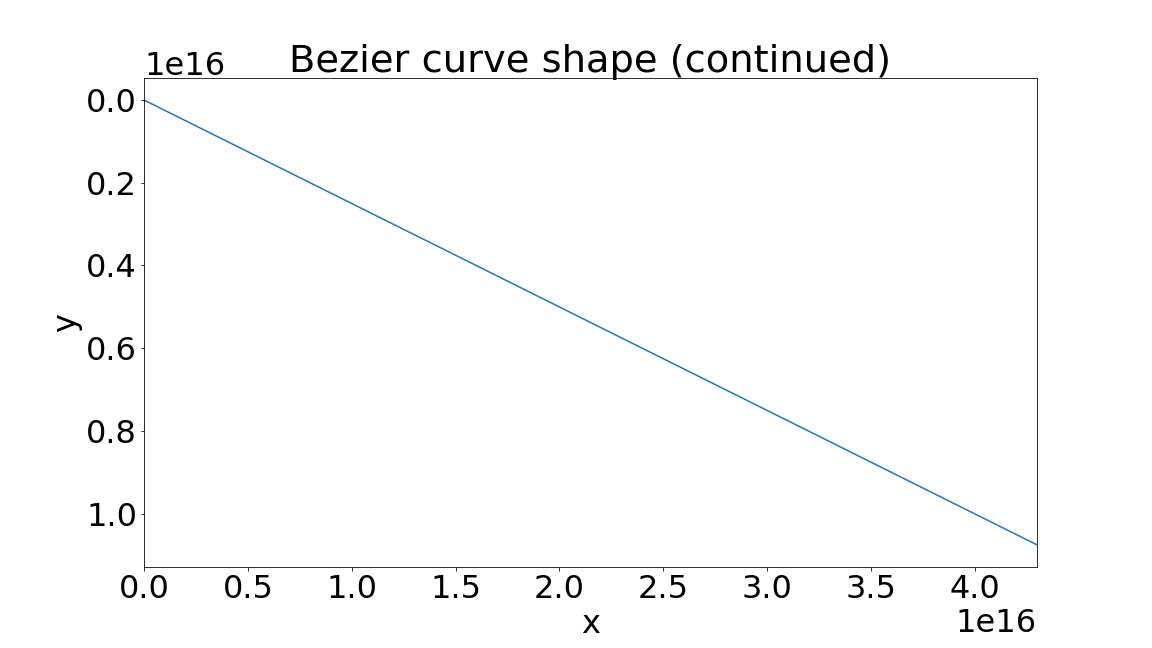
\includegraphics[width=1.00\textwidth]{images/bezier-curve-2.png}
  }
\end{frame}

\againframe{od-table}

\begin{frame}{Data (again)}
  \only<1>{
    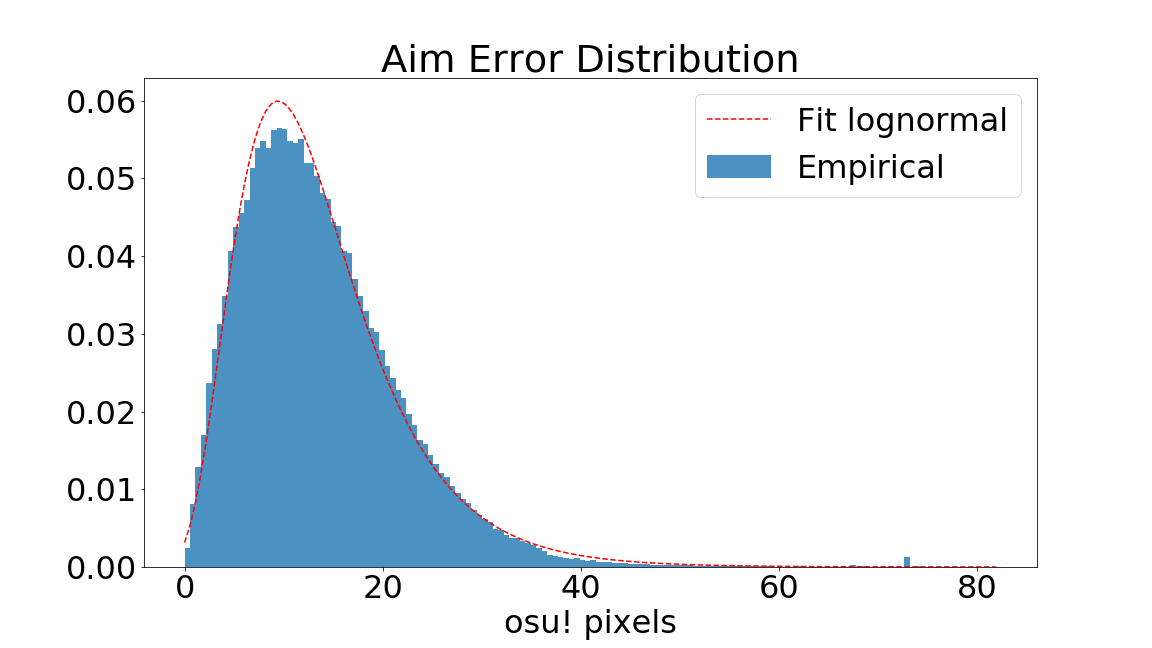
\includegraphics[width=1.00\textwidth]{images/aim-error-dist.png}
  }

  \only<2>{
    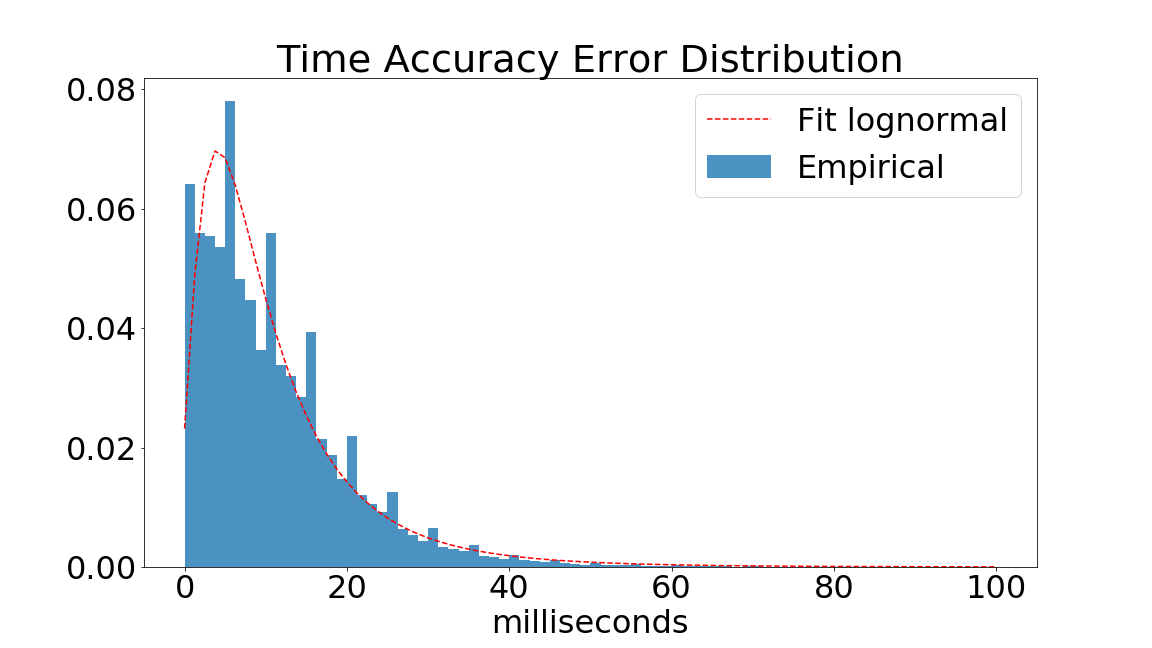
\includegraphics[width=1.00\textwidth]{images/accuracy-error-dist.png}
  }
\end{frame}

\begin{frame}{Fit a distribution}
  \texttt{lain/lstm.py:605}
\end{frame}

\begin{frame}{Sample Weights}
  \only<1>{
    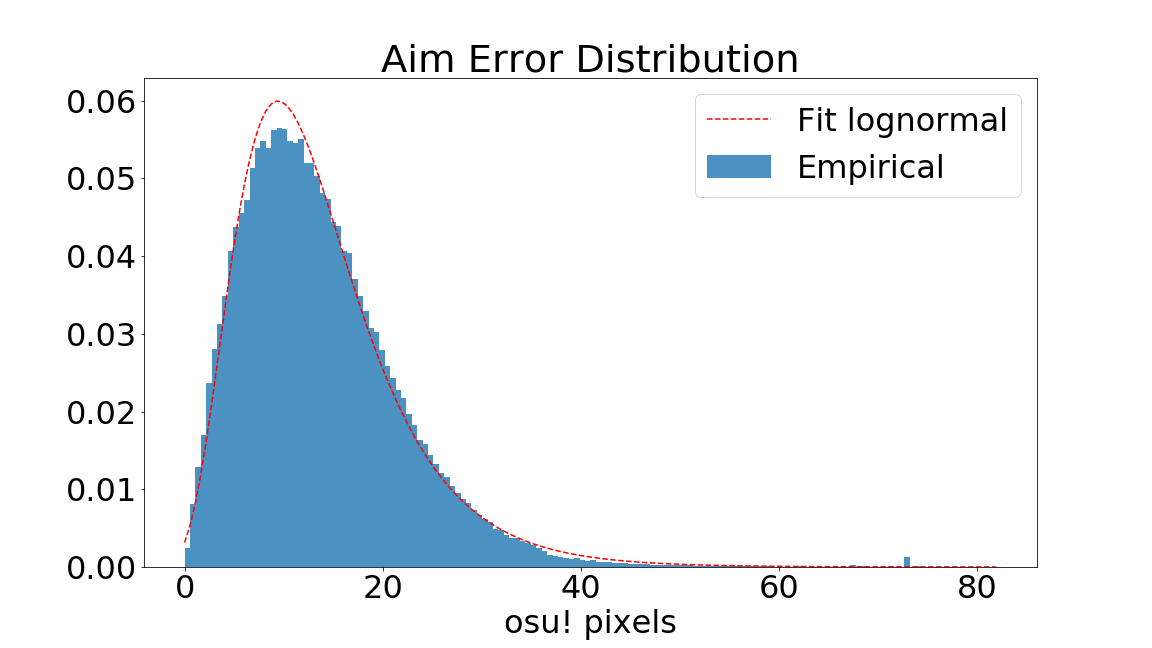
\includegraphics[width=1.00\textwidth]{images/aim-error-dist.png}
  }

  \only<2>{
    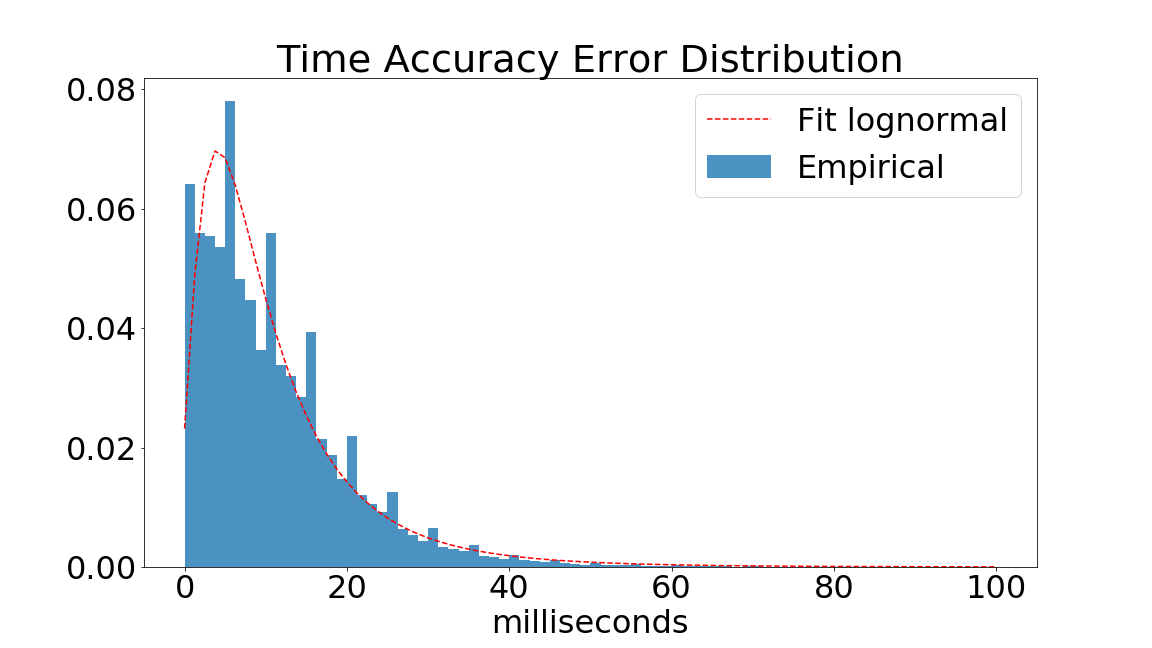
\includegraphics[width=1.00\textwidth]{images/accuracy-error-dist.png}
  }
\end{frame}

\begin{frame}[fragile]{Sample Weights (cont.)}
  \begin{minted}{python}
model.fit(
    ...
    {
        'aim_error:': aim_error_weights,
        'accuracy_error': accuracy_error_weights,
    },
)
  \end{minted}
\end{frame}

\begin{frame}{Example Output}
  \only<1>{
    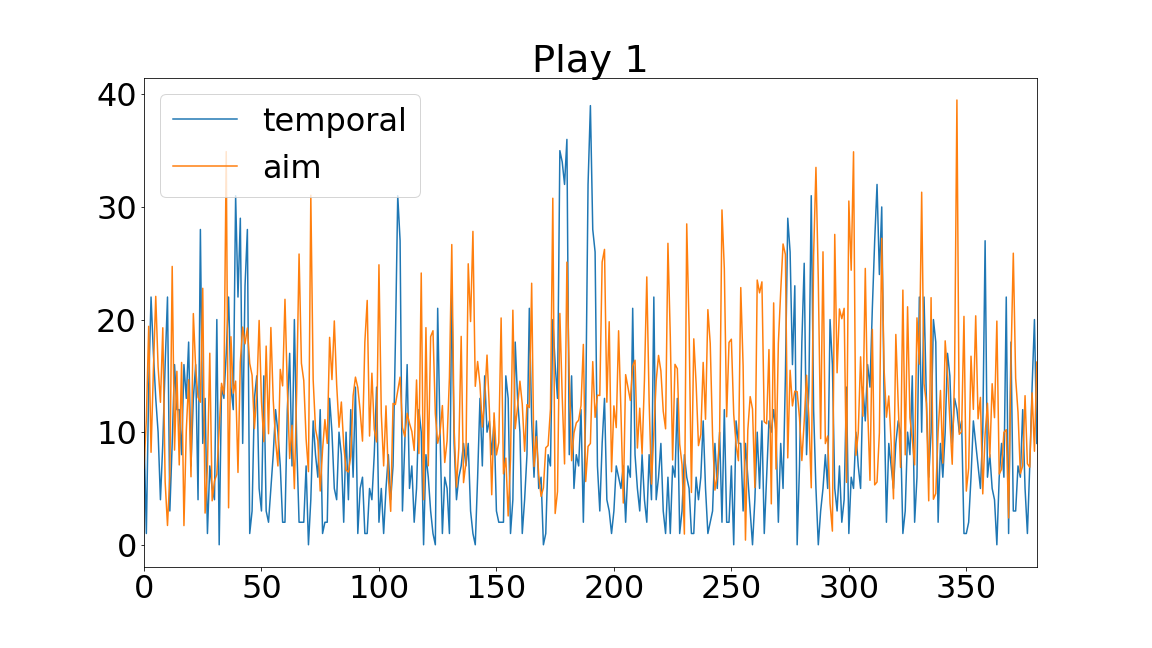
\includegraphics[width=1.00\textwidth]{images/play-1.png}
  }

  \only<2>{
    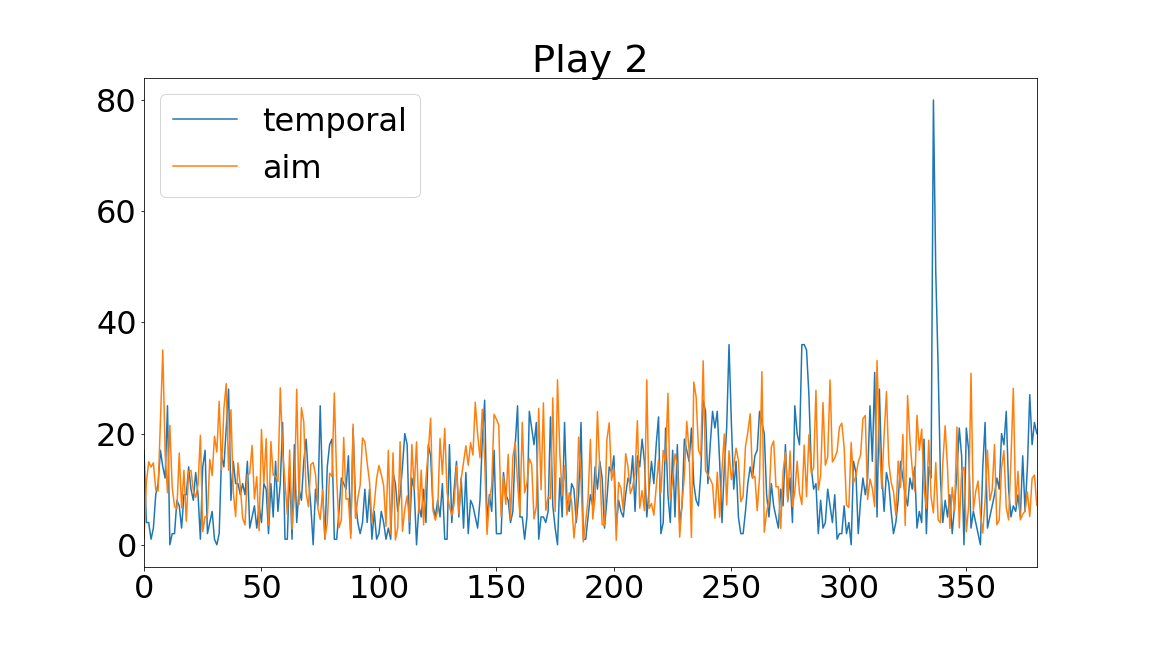
\includegraphics[width=1.00\textwidth]{images/play-2.png}
  }

  \only<3>{
    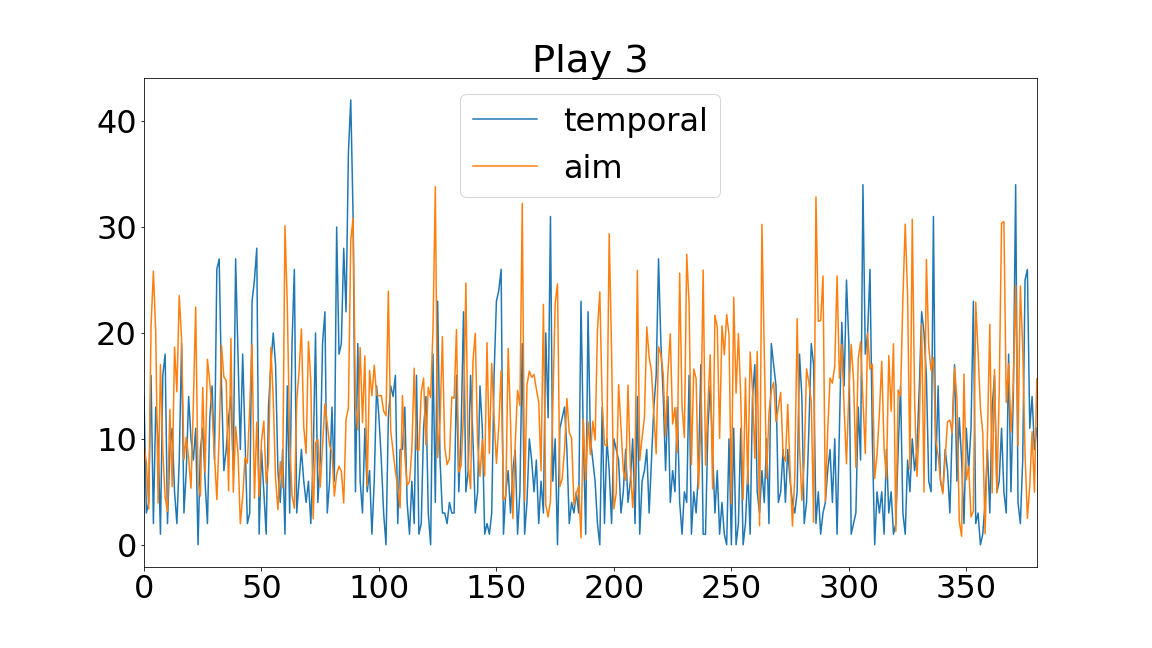
\includegraphics[width=1.00\textwidth]{images/play-3.png}
  }

  \only<4>{
    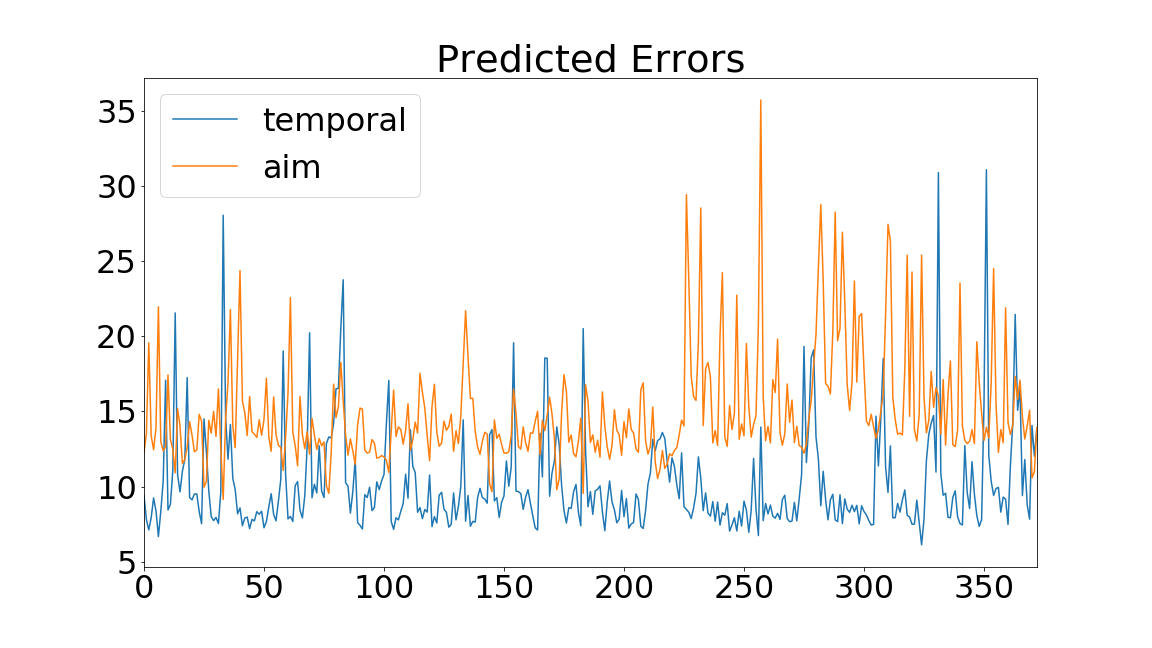
\includegraphics[width=1.00\textwidth]{images/predicted-errors.png}
  }
\end{frame}

\begin{frame}{Example Output (cont.)}
  \begin{center}
    \begin{tabular}{r | r | r}
      Prediction & Actual & Stars \\
      \hline
      99.85\% & 99.13\% & 5.34 \\
      99.85\% & 99.08\% & 5.34 \\
      99.85\% & 98.51\% & 5.34 \\
      95.95\% & 96.57\% & 6.03 \\
      98.30\% & 97.09\% & 6.24
    \end{tabular}
  \end{center}
\end{frame}

\section{Tips}

\begin{frame}{Understanding the process}
  \begin{itemize}
  \item[]<1-> \texttt{verbose} flags that log information
  \item[]<2-> progress indicators (\texttt{click.progressbar})
  \item[]<3-> print summary statistics early in process
  \end{itemize}
\end{frame}

\begin{frame}{Software Engineering Matters}
  Group code into a domain-aware \texttt{Model} class.

  \begin{itemize}
  \item[]<2-> feature extraction
  \item[]<3-> feature scaling
  \item[]<4-> label extraction
  \item[]<5-> managing keras
  \end{itemize}
\end{frame}

\begin{frame}{Serialization}
  \begin{itemize}
  \item[]<1-> save models to disk
  \item[]<2-> train on ec2 and use locally
  \item[]<3-> train locally then deploy
  \item[]<4-> supported by keras
  \end{itemize}
\end{frame}

\begin{frame}{Key Points}
  \begin{enumerate}
  \item<1-> Most of the work is before or after keras
  \item<2-> Understand the data and the data collection processes
  \item<3-> Osu! is a fun game
  \end{enumerate}
\end{frame}

\begin{frame}{Thank You}
  Questions?

  \begin{center}
    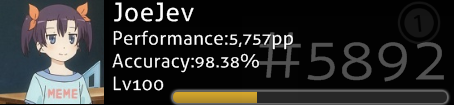
\includegraphics[width=0.50\textwidth]{images/osu-profile.png}
  \end{center}

  \begin{block}{\texttt{github.com/llllllllll} (10 lowercase L's)}
    \begin{itemize}
    \item \texttt{/lain} (model implementation)
    \item \texttt{/slider} (tools for working with osu! data and API)
    \item \texttt{/combine} (irc server running lain-as-a-service)
    \end{itemize}
  \end{block}
\end{frame}

\end{document}